\chapter{Infeasibility Gliding in Compositional Spaces} \label{chap:infeasibilitygliding}

\acknowledge{
This chapter adapts parts of a manuscript draft planned for future publication, co-authored with Arindam Debnath, Shuang Lin, Alexander Richter, Ricardo Amaral, Wesley F. Reinhart, Allison M. Beese, and Zi-Kui Liu. All of included text was written by Adam M. Krajewski. Described software has been developed by Adam M. Krajewski extending \texttt{nimplex} described in Chapter \ref{chap:nimplex} and used to generate results employing thermodynamic models developed by Shuang Lin. All other authors provided edits and guidance.
}

\section{Introduction} \label{infglide:sec:intro}

As explored in Chapter~\ref{chap:nimplex}, exploration of high-dimensional compositional spaces, needed for many materials discovery tasks, is a challenging task both conceptually and computationally, due to several inherent complexities. Typically, this forces efforts like screening and path planning to include as much prior knowledge (i.e., assumptions) as possible to bring these complexities down as much as possible, what has been explored in detail in Section~\ref{nimplex:ssec:complexes} on three individual examples.

It is important, however, to note that the assumptions imposed on the design space to reject spaces unlikely to work, like "\textit{Boron cannot be added because it will precipitate borides}", by the same assumptions do not significantly increase the volume of feasible (or desired) space. Thus, an approach that would explore only such regions, while skipping the rest, could in principle consider such design space at a low additional cost, reducing the number of assumptions and possibly identifying high-performing materials that would otherwise be skipped.

\section{Exploiting Compositional Graph Representation} \label{infglide:sec:exploitgraph}



\begin{figure}[H]
    \centering
    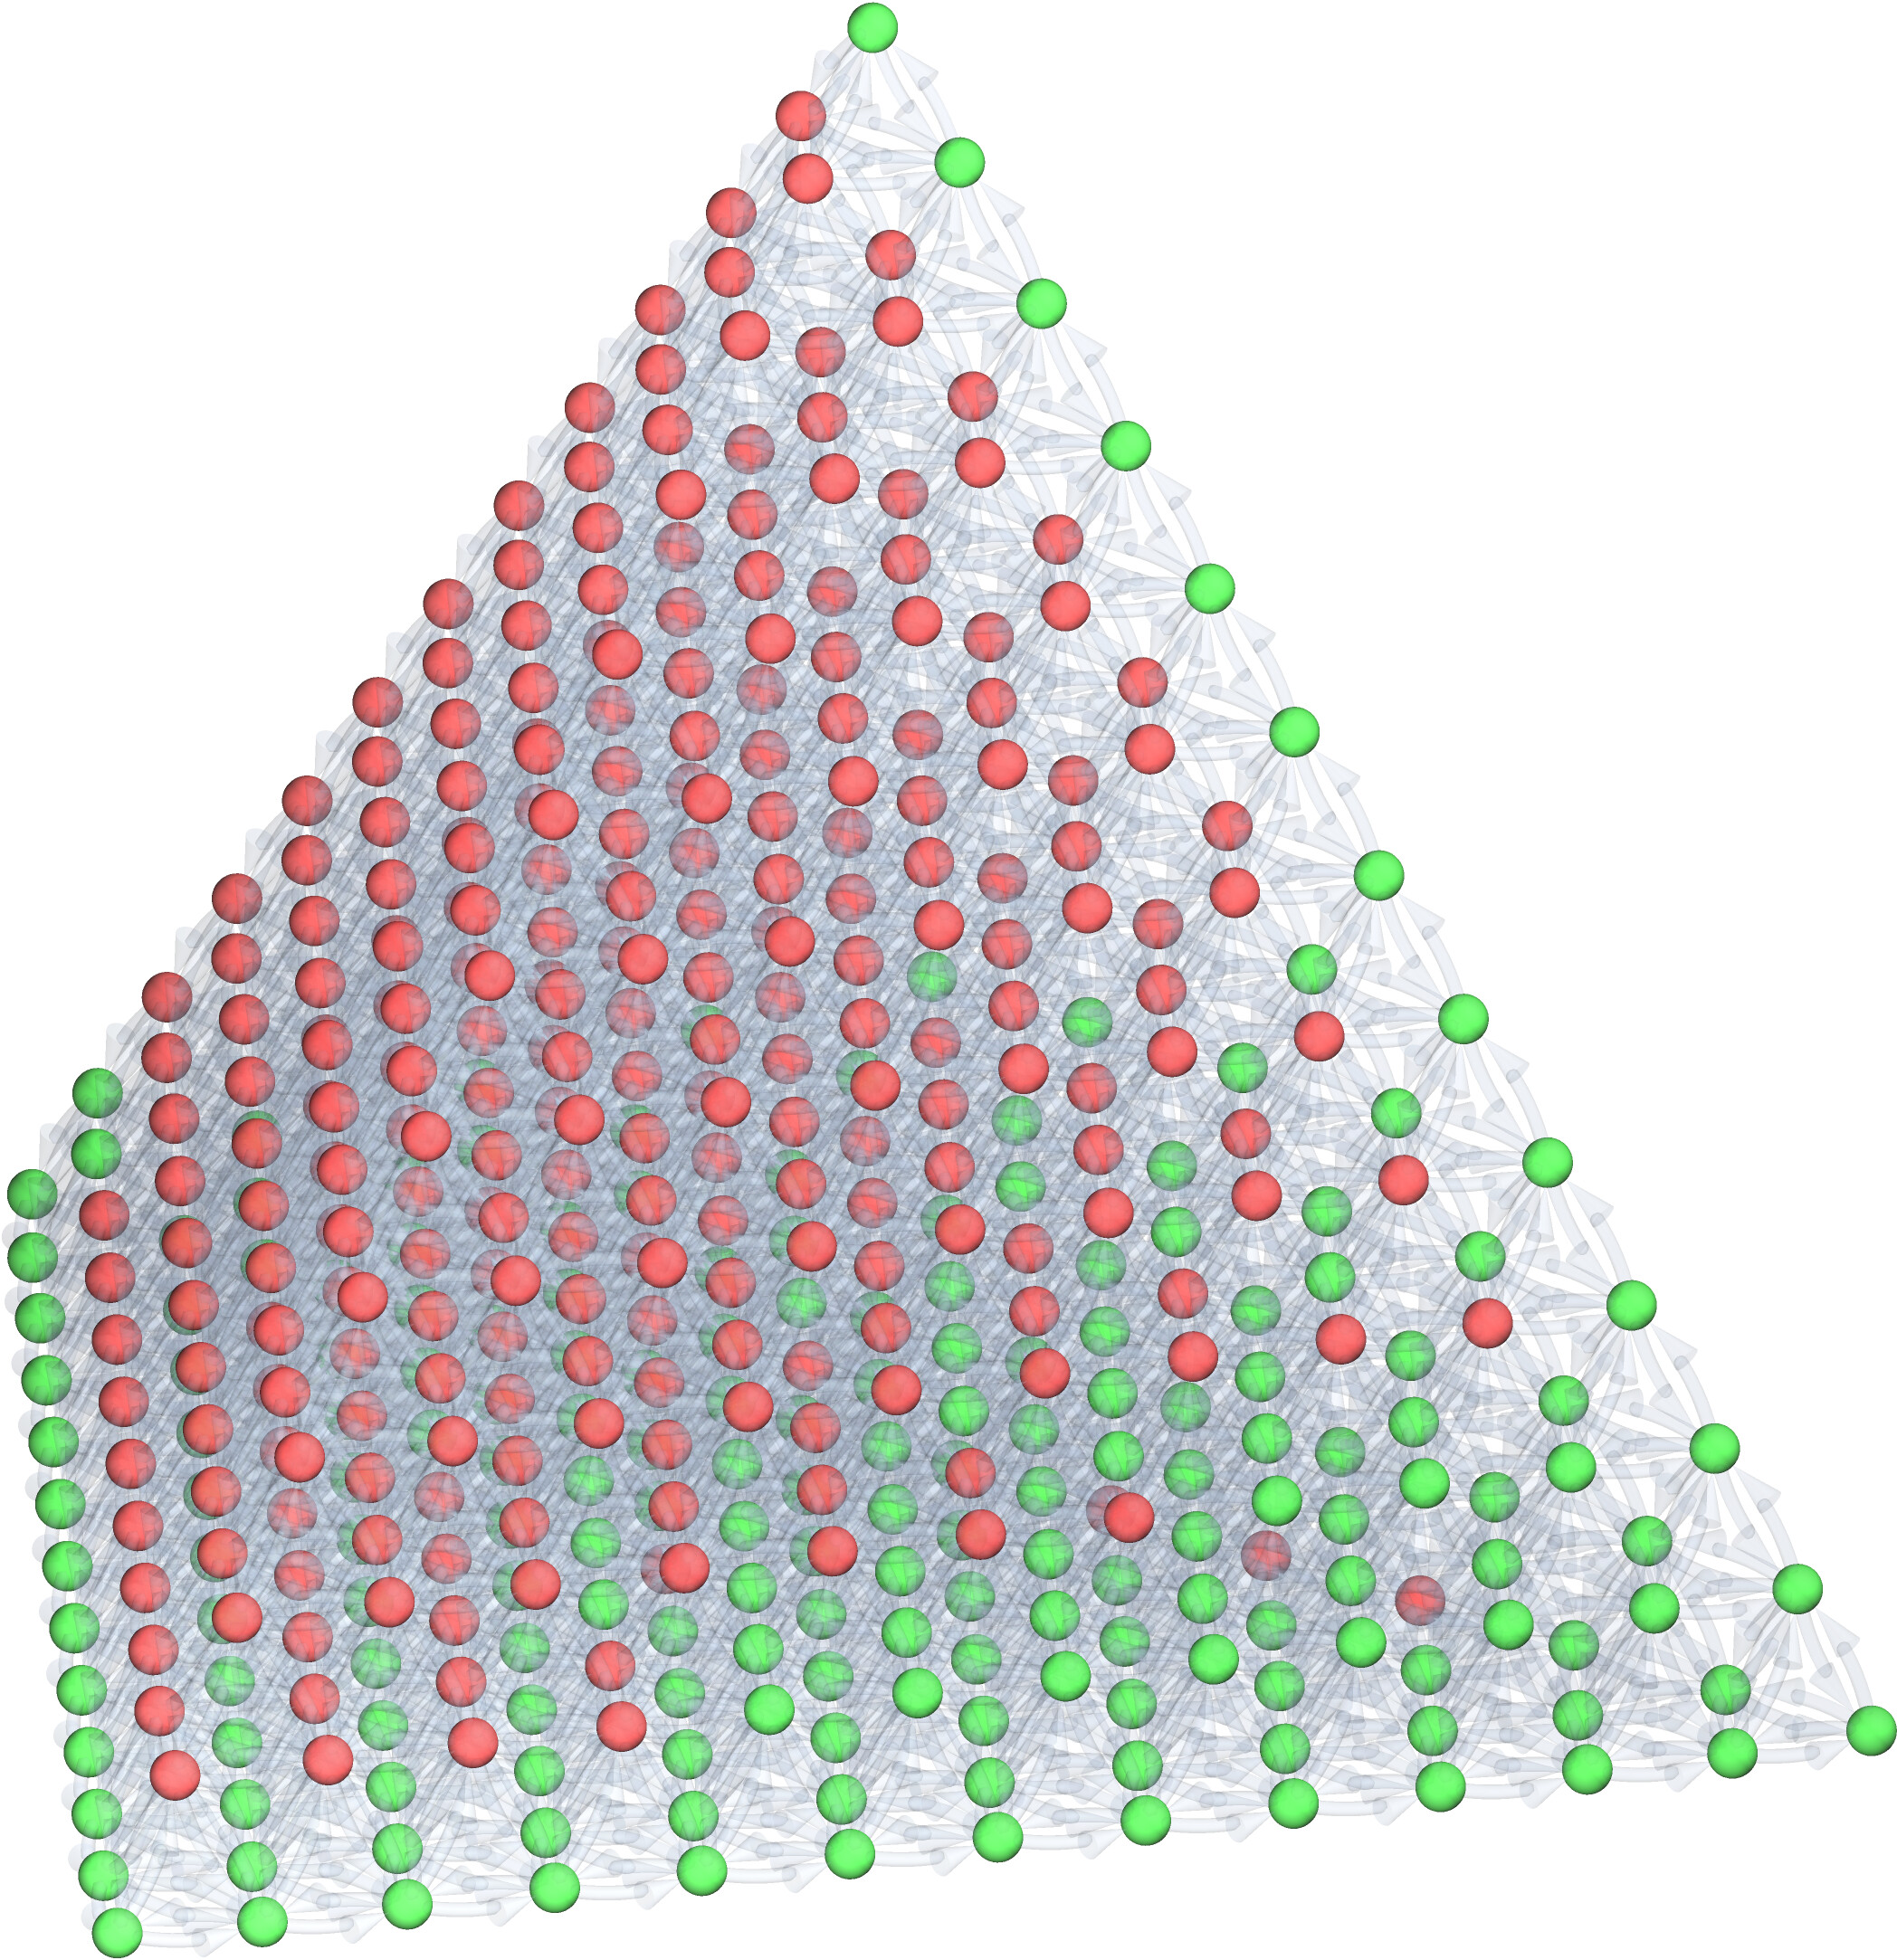
\includegraphics[width=0.7\textwidth]{infeasibilitygliding/InfeasibilityGliding_Full.png}
    \caption{Feasibility map over compositional tetrahedron (3-simplex) formed by all combinations of Ti50 Zr50, Hf95 Ti5, Mo33 Nb33 Ta33, Mo80 Nb10 W10 discretized at 12 divisions per dimension. The positions in the 7-component elemental space obtained from \texttt{nimplex}, described in Chapter \ref{chap:nimplex}, were used to run \texttt{pycalphad} \cite{Otis2017Pycalphad:Python} evaluations and constrained by limiting phases present at equilibrium at 1000K to single or many solid solution phases. Roughly half of the compositions are infeasible with most of them forming a single large region.}
    \label{infeasibilitygliding:fig:fullcomputation}
\end{figure}



\section{Gliding on the Boundaries of Infeasibility} \label{infglide:sec:glide}

\subsection{Underlying Assumptions} \label{infglide:ssec:assumptions}

\todo

\begin{figure}[H]
    \centering
    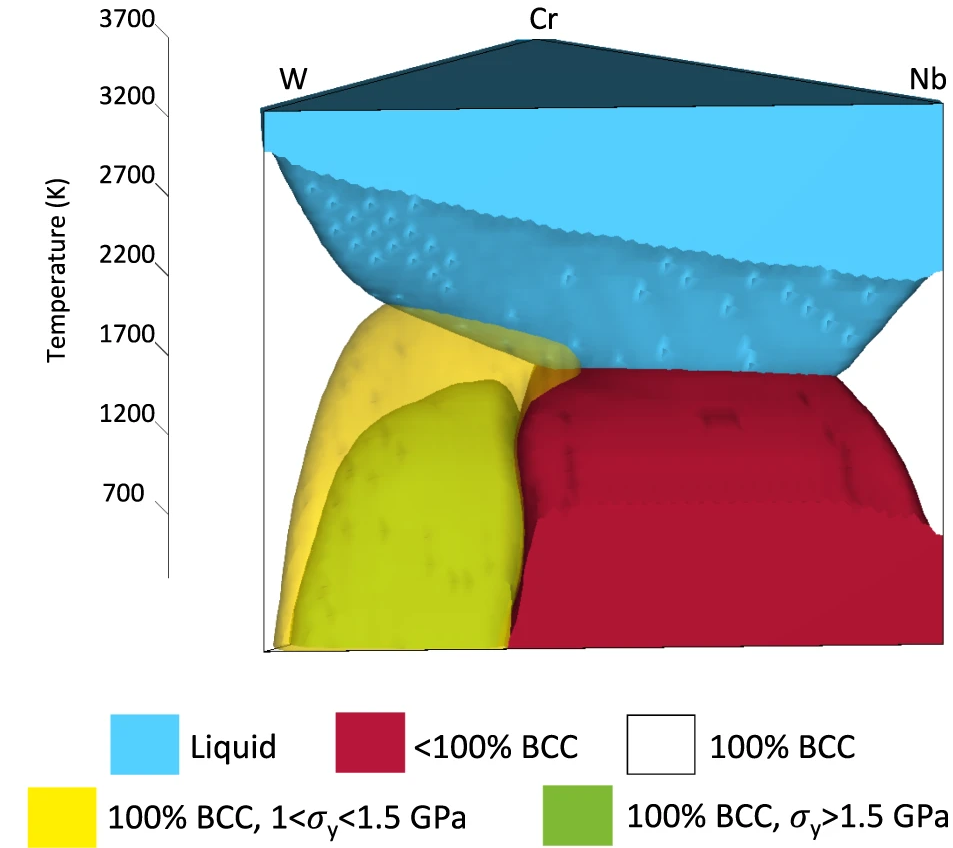
\includegraphics[width=0.5\textwidth]{infeasibilitygliding/PhaseTernaryMap_Elder2023.png}
    \caption{A view of ternary Cr-Nb-W phase diagram projected across a temperature range of phase classes, further augmented by imposing predicted property value constraints. It depicts the smoothness of the infeasible region boundary (red) and increasingly smooth boundary of property-constrained region. Taken from Figure 2b in \citet{Elder2023ComputationalValidation} under CC BY 4.0 license.}
    \label{infeasibilitygliding:fig:katesphasemap}
\end{figure}


\subsection{Unbiased Exploration Searches} \label{infglide:ssec:unbiasedexplore}

\todo 

\begin{figure}[H]
    \centering
    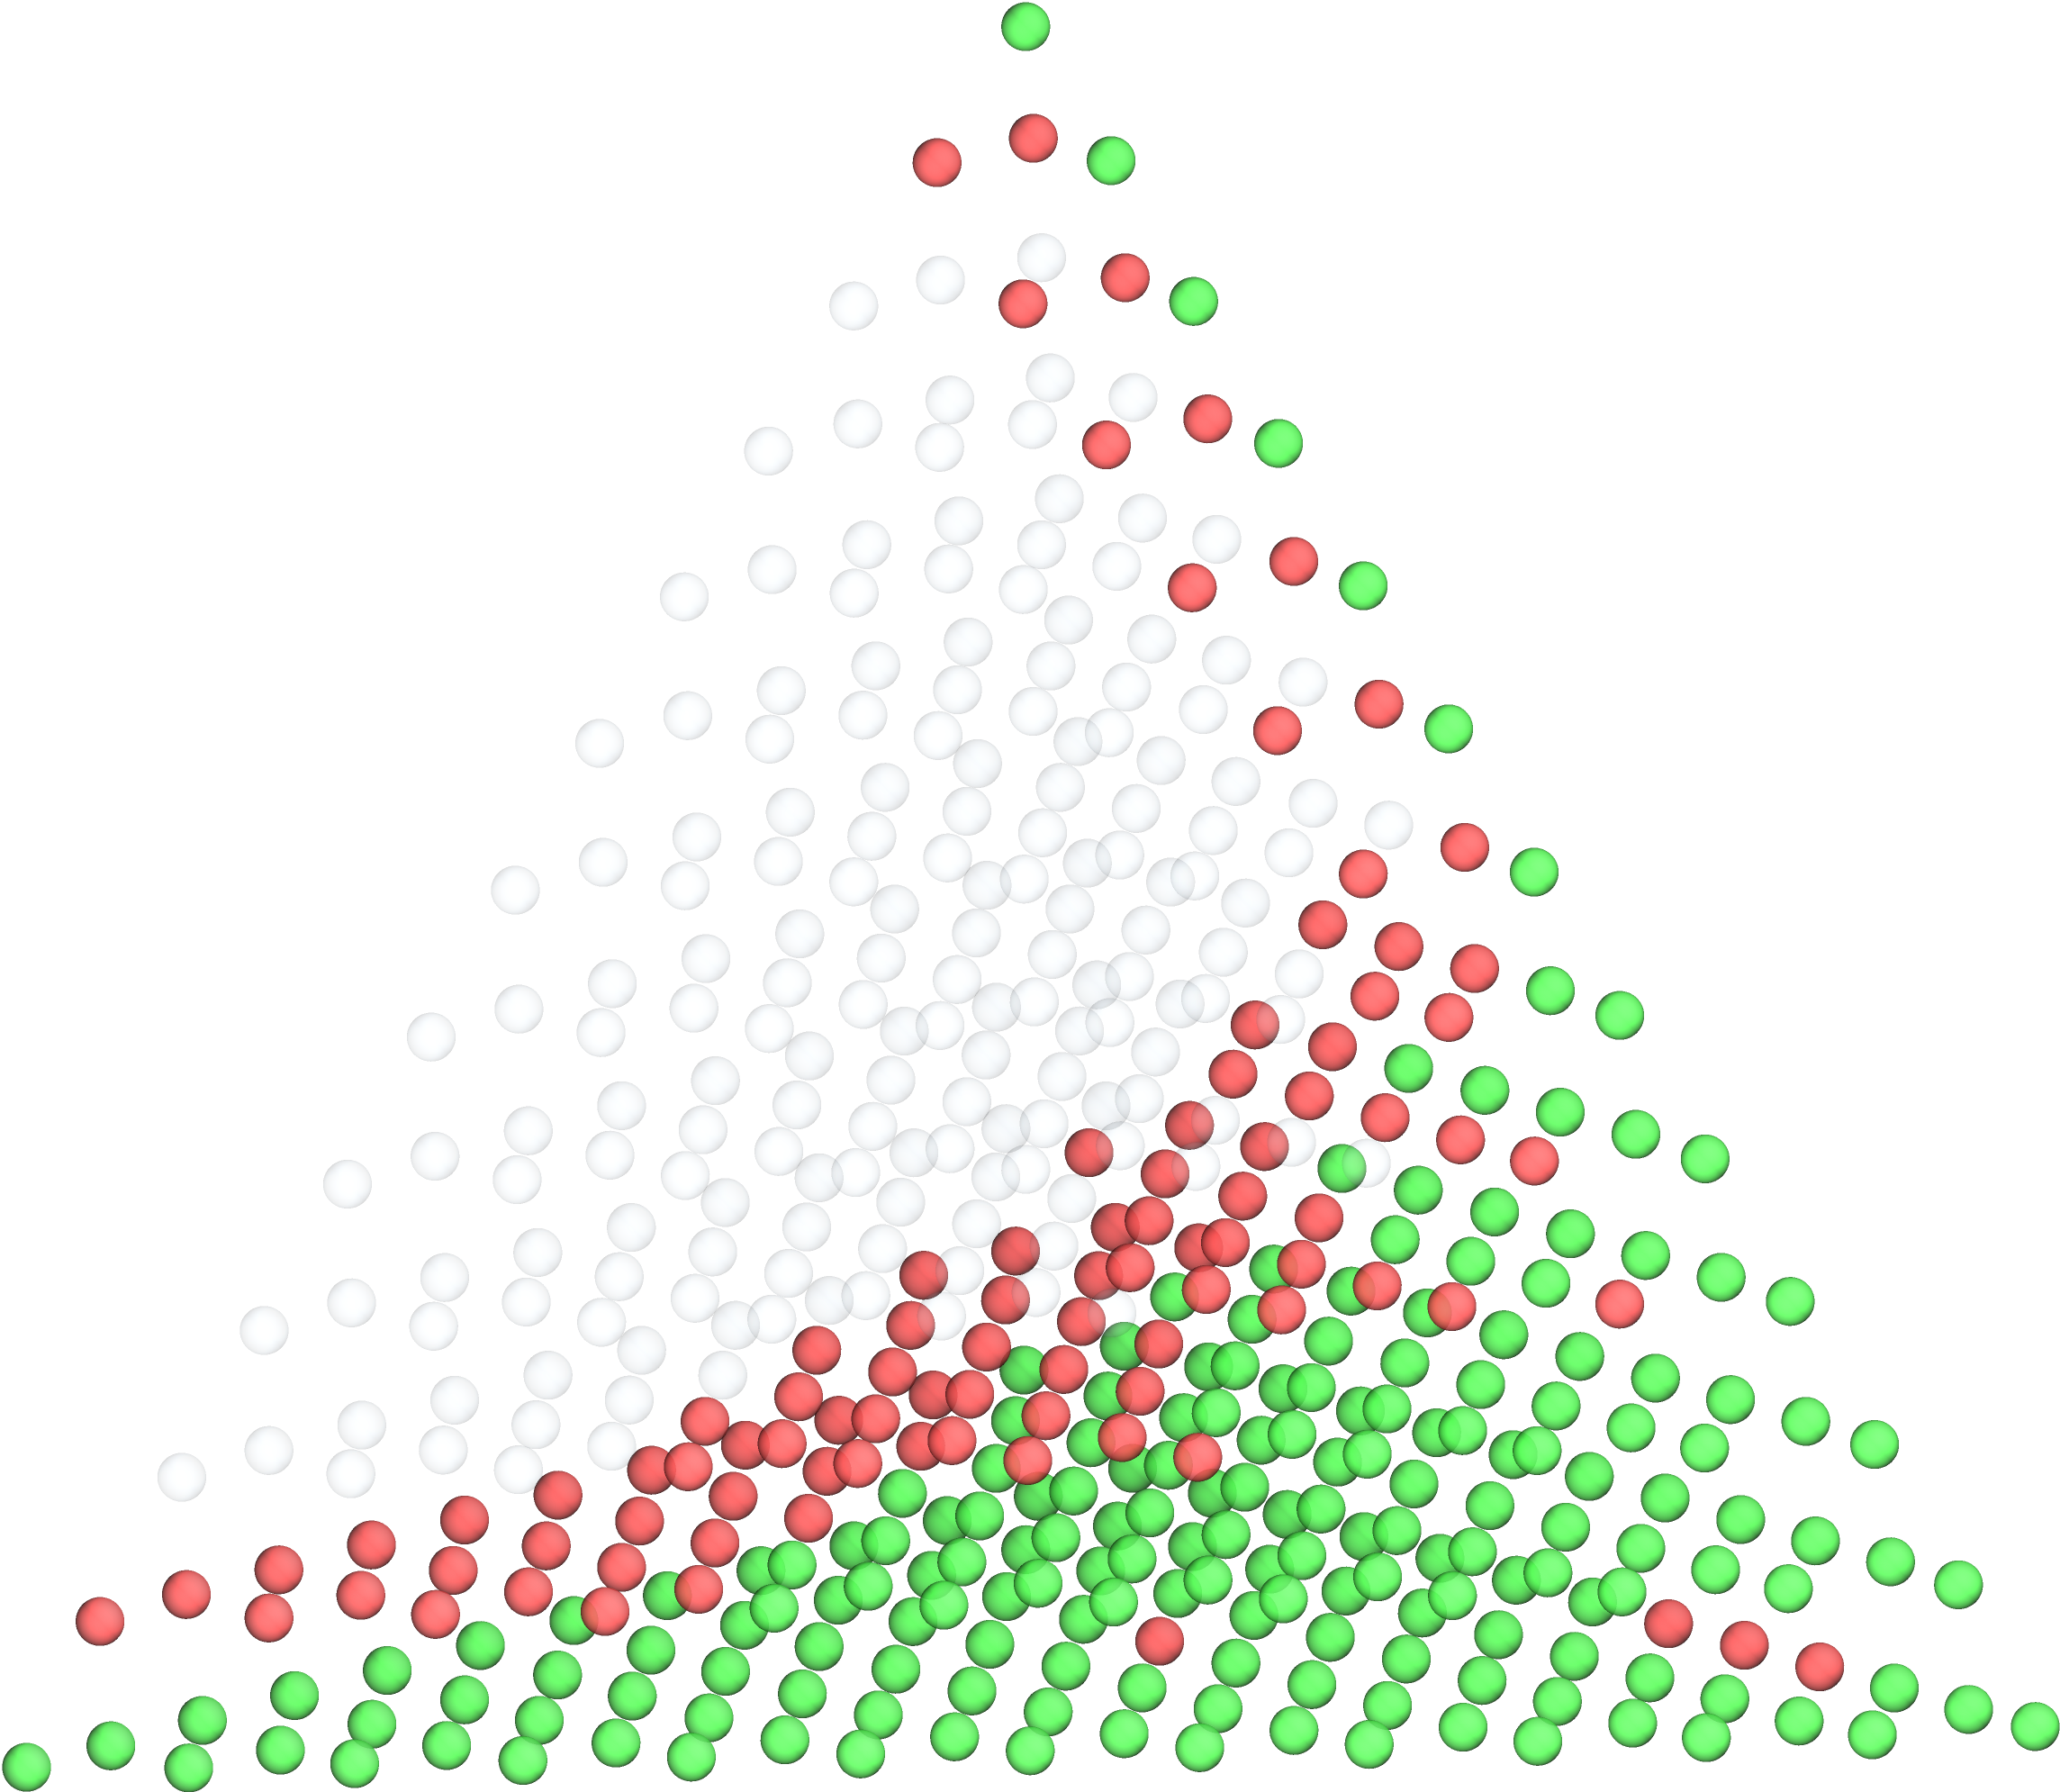
\includegraphics[width=0.7\textwidth]{infeasibilitygliding/InfeasibilityGliding_Glide.png}
    \caption{The same problem as in Figure \ref{infeasibilitygliding:fig:fullcomputation} solved by iteratively exploring all feasible paths in the compositional graph in depth-first approach, which can be started from one or multiple points, and terminated once goal is reached or once all of the feasible space is explored.}
    \label{infeasibilitygliding:fig:glide}
\end{figure}


\printbibliography[heading=subbibintoc]